\documentclass[../all.tex]{subfiles}
\begin{document}
%%%%%%%%%%%%%%%%%%%%%%%%%
\section{Experimentación} % Evaluación
%%%%%%%%%%%%%%%%%%%%%%%%%
	Una vez explicadas las tecnologías usadas y el marco del trabajo, se procederá a explicar detalladamente como se ha llegado a la resolución del trabajo detallando los procedimientos seguidos y justificando la elección de las librerías, algoritmos y técnicas usadas junto a los resultados obtenidos en cada una de las fases del proyecto.


\subsection{Problemática lenguaje natural}
	El procesamiento del lenguaje natural (PLN o NLP en sus siglas anglosajonas) es una rama de la Inteligencia Artificial encargada de estudiar métodos de comunicación entre máquina y hombre a través del lenguaje natural, es decir, el lenguaje empleado de forma habitual en una conversación escrita u oral entre personas.\\ 
	
	El lenguaje natural presenta muchas características que lo hacen un verdadero reto para las ciencias de la computación. Como suele pasar en el mundo de la Inteligencia Artificial, una tarea que puede parecer para una máquina. Aspectos como la ambigüedad, la espontaneidad, la falta de fluidez, las referencias y las abreviaturas son difíciles de procesar.

\subsubsection{Homonimia}
	La homonimia  es la cualidad de dos palabras, de distinto origen y significado por evolución histórica, que tienen la misma forma, es decir, la misma pronunciación o la misma escritura.\\
	
	Un ejemplo estaría en la palabra \textbf{vela}:
	\begin{enumerate}[resume]
		\setcounter{enumi}{0}
		\item Acción de velar; cilindro de cera con una mecha para iluminar. (Ambos sentidos relacionados con el verbo velar.
		\item Tela grande que aprovecha la fuerza del viento, especialmente en un barco.
	\end{enumerate}

	En castellano de homonimias tenemos diferentes clases:
	
	\begin{enumerate}[resume]
		\setcounter{enumi}{0}
		\item \textbf{Homónimos lexicales}: los que pertenecen a la misma categoría gramatical: onda y honda, botar y votar, haya y aya, ojear y hojear.
		\item \textbf{Homónimos gramaticales}: los que no pertenecen a la misma categoría gramatical: cabe verbo y cabe preposición, o los que perteneciendo a la misma categoría gramatical se diferencian en alguna marca morfemática: el pez, la pez; el orden, la orden.
		\item \textbf{Homónimos léxico-gramaticales}: los que se han formado a través de un cambio de funciones: poder (verbo) poder (sustantivo)
		\item \textbf{Homónimos morfológicos}: cuando se producen diferentes formas de una sola palabra: decía primera y tercera personas del pretérito imperfecto de indicativo; o se dan formas correspondientes de palabras diferentes: fui (de ser e ir); ve (de ir y de ver), etc.
	\end{enumerate}

\subsubsection{Polisemia}
	La polisemia, en lingüística, se presenta cuando una misma palabra o signo lingüístico tiene varias acepciones o significados. Una palabra polisémica es aquella que tiene dos o más significados que se relacionan entre sí.\\
	
	Cabe resaltar que la polisemia puede surgir por diversos motivos. Por un lado, el vocabulario figurado produce polisemia por medio de las metáforas y las metonimias. Por ejemplo: los brazos de un río, las patas de una mesa. La especialización y el lenguaje técnico también atribuyen un significado específico a ciertos términos (como en el caso del ratón en la informática).\\
	
	La influencia extranjera y las modificaciones de aplicación son otras condiciones que favorecen la polisemia: una muestra de esto es el vocablo botón que nació con la indumentaria y luego pasó a utilizarse también en los artefactos electrónicos.\\
	
	Un ejemplo estaría en la palabra \textbf{cabo}:
	\begin{enumerate}[resume]
		\setcounter{enumi}{0}
		\item (masculino) Punta de tierra que penetra en el mar.
		\item (masculino/femenino) Escalafón militar.
		\item (masculino) Cuerda en jerga náutica.
	\end{enumerate}
\newpage
\subsubsection{Anáfora y elipses}
	La anáfora se puede definir como la palabra o palabras que asumen el significado de una parte del discurso (texto) que ya se ha mencionado antes.\\
	
	Un ejemplo de anáfora sería:
	\begin{itemize}[resume]
		\item Estoy de paso por Madrid. {\small(Madrid)} Es maravillosa. 
	\end{itemize}
	Cuando el elemento sustituido aparece después del sustituto, hablamos de catáfora.\\
	Un ejemplo de catáfora sería:
	\begin{itemize}[resume]
		\item Quería estar con \underline{Jesús}; pero no \underline{lo} he visto en toda la tarde. 
	\end{itemize}

	Por otro lado tenemos las elipses que es la omisión o supresión de una o varias palabras que ya se habían mencionado antes o que se pueden presuponer o sobreentender. Esta construcción evita el uso de repeticiones innecesarias.\\
	Un ejemplo de elipse sería:
	\begin{itemize}[resume]
		\item El concierto fue genial, la comida {\small(fue)} regular. 
	\end{itemize}
\subsubsection{Sintaxis no normalizada}
	 Otro problema que nos plantea el análisis de lenguaje natural es el hecho de que su estructura no está normalizada, es decir, a la hora de utilizar el lenguaje en español, no se utiliza una sintaxis concreta y bien definida, si no que a la hora de expresar una misma idea, ésta se puede estructurar de diversas maneras.
 	\begin{itemize}[resume]
	 	\item Me encantan las mañanas de domingo.
	 	\item Las mañanas de domingo me encantan.
 	\end{itemize}
	 Ambas oraciones expresan la misma idea utilizando un orden diferente en las distintas palabras que las componen.
\newpage
\subsubsection{Contexto}
	El contexto es el conjunto de circunstancias (materiales o abstractas) que se producen alrededor de un hecho, o evento dado, que hacen que una palabra pueda tomar varios sentidos según el momento en el cual se utiliza.\\
	
	Un claro ejemplo de la importancia del contexto es la ironía, a un suceso malo se puede contestar con otra frase 'mala' como sería el caso de; \textit{¡Otra vez no!}, con una frase buena del estilo; \textit{¡Qué bien!} donde estaríamos siendo irónicos o con una frase como; \textit{¿Porqué a mí?}.
	
\subsubsection{Otras circunstancias}

	Aparte de toda esta serie de fenómenos que se dan en la lengua formal, hay que tener que cuenta otros aspectos que se dan en ambientes más coloquiales como son las redes sociales.\\
	
	En la siguiente tabla se muestran algunos ejemplos de cómo un mismo mensaje puede tener formas diferentes según el usuario y el medio en el que lo escriba.
	\begin{center}
		\begin{tabular}{ | m{7cm}| m{7cm} | } 
			\hline
			\textbf{Texto de ejemplo} & \textbf{Explicación}\\ 
			\hline
			Messi es el mejor jugador de la historia del fútbol. & Frase correcta \\ 
			\hline
			Mesi es el mejor jugador de la istoria del futbol; & Faltas de ortografía\\ 
			\hline
			MesSi es el MeJor juGAdor de la hIStoriA del fúTBol :) & Incluir mayúsculas y símbolos innecesarios\\ 
			\hline
			Messiiii es el mejor jugador de la historia del futbooooool & Añadir repetición de letras para darle mayor énfasis a la palabra\\ 
			\hline
			Mssi s l mjor jugadr d la histria dl futbol  & Lenguaje SMS.\\ 
			\hline
			¡Vamos equipo! & Brevedad y ambigüedad del texto \\ 
			\hline
		\end{tabular}
	\end{center}

\newpage
\subsection{Fase 0 - Extracción de la información}
	{\color{red} 
		TODO: Falta adjuntar los resultados
	}

\newpage
\subsection{Fase 1 - Clasificación de texto según temática}


\begin{figure}[H]
    \centering
    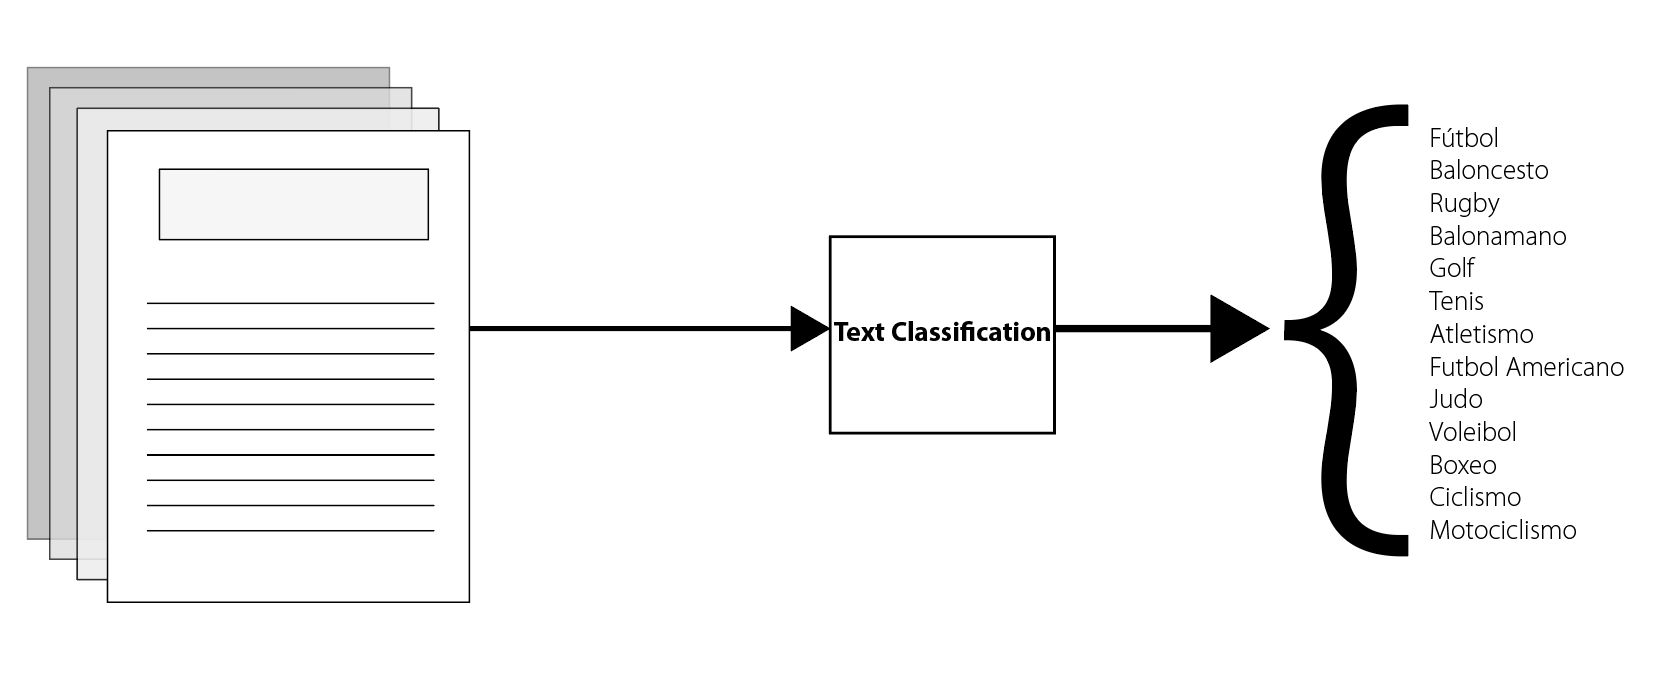
\includegraphics[height=13cm, width=15cm]{imgs/textClassification.png}
    \caption{Idea principal del clasificador de texto}
\end{figure}


Para está primera fase primero se quiso evaluar según el contenido de Wikipedia. Se extrajeron las palabras más repetidas del contenido de cada deporte en Wikipedia. Para ello se quitaron los signos de puntuación y palabras vacías, entendiendo como palabras vacías todos los artículos, preposiciones y números. {\color{red} TODO: adjuntar foto resultado}\\

Con esta técnica se pudo ver que funcionaba bien para clasificar textos grandes como artículos o noticias pero en frases cortas como son los \textit{tweets} no se conseguía una \textit{accuracy} que se pudiera considerar aceptable. Para mejorarlo se decidió hacer una ontología de cada uno de los deportes. En concreto se decidió clasificar las palabras que envolvían un deporte según tres criterios; \textit{key words} que son las palabras que solo se utilizan en un deporte, sus jugadores más destacados y los nombres de sus campeonatos (ej: fútbol; Lionel Messi, bota de oro, etc), \textit{secondary words} que son palabras que se pueden usar en ese deporte pero que pueden referir a algún otro deporte (ej: fútbol; balón, pelota, botas, etc) y por último \textit{excluding words} que son todas las \textit{key words} de los otros deportes y \textit{secondary words} de otros deportes que excluyen (ej: fútbol; manillar, palo de hierro, etc).\\

Se intento hacer stemmer pero empeorava los resultados, lo probaremos otra vez en analisis del sentimiento
se hizo con wiki, por  diccionario propio y para mejorar los tiempos con diccionario propio y arbol

\begin{figure}[H]
    \centering
    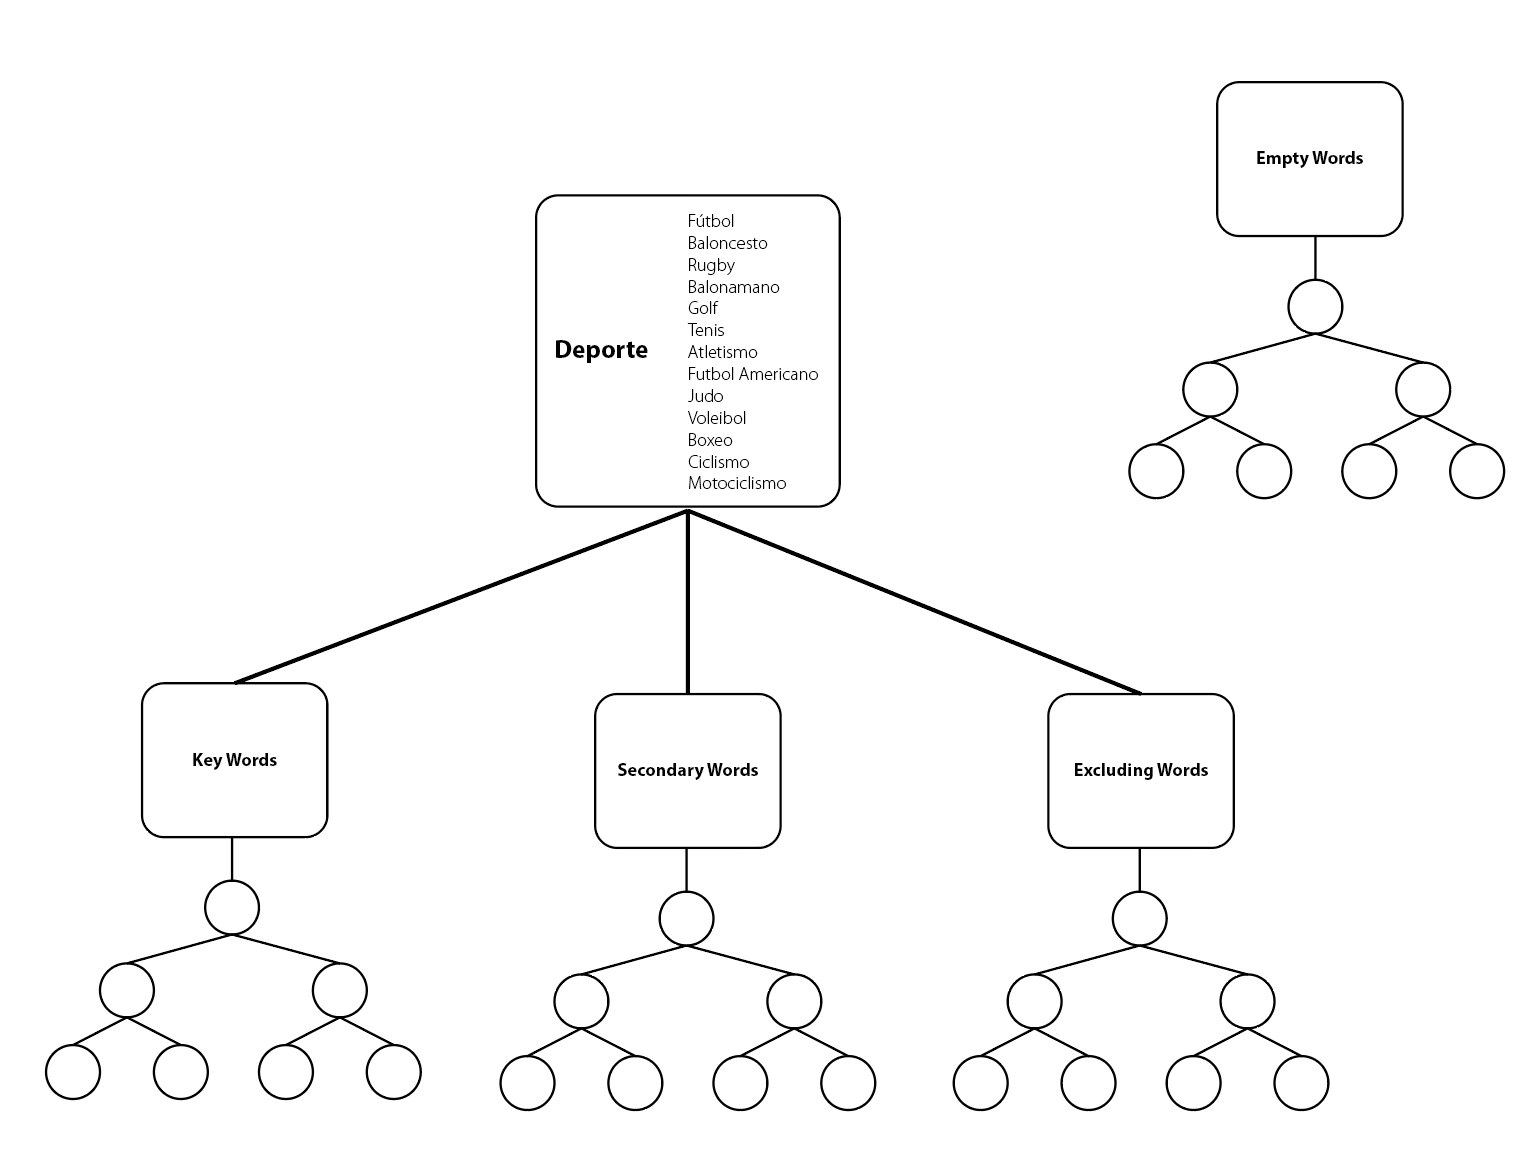
\includegraphics[height=13cm, width=15cm]{imgs/treeScheme.png}
    \caption{Esquema estructuración de los datos}
\end{figure}

{\color{red} 
    TODO: TABLA COMPARATIVA DE LOS METODOS y Faltan los resultados
}
\newpage
\subsection{Fase 2 - Análisis del sentimiento}
    El análisis de sentimiento de textos en las redes sociales (que adopta diferentes nombres en inglés como sentiment analysis, opinion mining, brand monitoring, buzz monitoring, online anthropology, market influence analytics, conversation mining, online consumer intelligence, user generated content) es el proceso que determina el tono emocional que hay detrás de unas palabras determinadas, si una frase contiene una opinión positiva o negativa sobre un producto, marca, institución, organización, empresa, evento o persona.\\
    
    Palabras difíciles\\
    
    Los sentimientos se clasifican en positivos, negativos o neutros. Sin embargo, el lenguaje natural es complejo y ambiguo por lo que enseñar a una máquina a que analice los diferentes matices gramaticales, variaciones culturales, jergas, expresiones coloquiales o a distinguir faltas de ortografía, la sinonimia o la polisemia dentro de un contexto que determina el tono de la conversación es francamente difícil. Así, por ejemplo, ante un comentario sarcástico, la máquina tomaría la frase como algo positivo en vez de algo negativo o expresiones como “LOL, OMG, estuvo geeeeeeeniaaaaaaaal” son dificilísimas de procesar.\\
    
    
    
	{\color{red} 
		TODO: Faltan los resultados, COMENTAR QUE SI EL STEMMER FUNCIONASE MEJOR EN ESPAÑOL MEJORES RESULTADOS
	}
\newpage
\subsection{Fase 3 -}

\url{http://www.outono.net/elentir/2013/02/02/twitter-5-formas-de-identificar-a-un-troll-y-5-consejos-para-librarte-de-el/}
\url{https://www.fucsia.co/opinion/blogs/entrada-blog/como-detectar-mentiras-internet/35060}
\url{https://www.biobiochile.cl/noticias/2013/09/16/3-senales-para-detectar-cuando-te-mienten-en-facebook-o-whatsapp.shtml}
\url{https://www.elconfidencial.com/tecnologia/2014-02-27/pheme-un-detector-de-mentiras-para-las-redes-sociales_94300/}

\newpage
\subsection{Utilización de la aplicación}

\end{document}
